%%%
%%% performance.tex
%%%

\subsection{Performance Evaluation}
\label{sec:performance}


In this section, we evaluate the performance of our implementation of
the BGP emulator.  We do not attempt to perform a complete performance
analysis of the prototype.
% our goal is not to analyze performance
%bottlenecks or optimize the running times of our algorithms of our
%particular implementation of the BGP emulator. 
Rather, we conduct
experiments that demonstrate the {\em practicality} of the prediction
algorithm.  

While our evaluation is preliminary, our performance tests demonstrate
that the emulator can operate on timescales that could allow an operator
to use a 
BGP emulator based on our algorithms in a practical setting.  
%While our evaluation is preliminary, it
%demonstrates the efficiency of the BGP emulator and its prediction
%algorithms, especially for common operations such as incremental
%configuration changes. 
Our evaluation demonstrates the
following points:
\begin{itemize}
\item The emulator computes the best routes for one prefix throughout a
  large tier-1 ISP network in about one second.  Although predicting the
  best route for all prefixes at all routers in such a
  network takes several hours, this type of computation does not need to
  be performed all that frequently in practice.
\item Exploiting commonalities among route advertisements
  to eliminate redundant computation reduces
  the running time of the emulator by approximately 50\%.
\item Using the emulator to evaluate the effects of an incremental
  change to router configuration typically takes only a few seconds.
  Thus, we believe that the emulator can be practical for tasks
  such as interdomain traffic engineering.
\end{itemize}


After briefly discussing the evaluation framework, we examine the
emulator's performance.  First, we discuss the emulator's performance
when it computes the routes for {\em every} prefix in the routing table
from scratch, without any performance optimizations.  We then examine
how insights from the BGP decision process and previous measurement
studies can improve performance.  Finally, we describe how the emulator
can quickly predict the effects of incremental configuration changes.
% and
%examine the emulator's performance when computing these incremental
%changes.



\subsubsection{Evaluation Framework}

We ran the emulator on a Sun Fire 15000 with 192 GB of RAM and 48
900 MHz Ultrasparc-III Copper processors.  Because this is a time-shared
machine, we ran each of our experiments several times to ensure the
accuracy of our measurements.  Except where noted, the prototype used
only two 900 MHz processors (one for the database process and one for
the emulator itself); the combined memory footprint of the
database process and the emulator never exceeded 50 MB.  Because the
emulator did not use more resources than a standard PC, the results of
our evaluation should reasonably reflect the emulator's
performance on commodity hardware.

%[stress that we'll report memory usage info, and we explicitly
%use just one CPU except where noted]
%% We evaluated running times for data sets of various sizes and scenarios
%% to demonstrate that the emulator is efficient enough to be used in
%% practice, even on a large AS such as AT\&T's commercial IP backbone.
%% Most ASes have fewer BGP sessions, peers, and routers, and perhaps fewer
%% prefixes.  To quantify the overhead of running the emulator for a small
%% number of sessions, we run the emulator on scenarios with just one or
%% two eBGP sessions.  For the one-session experiment, we select one of the
%% eBGP sessions responsible for the largest number of routes in the AT\&T
%% network.  For the two-session experiment, we include an eBGP session at
%% the same router of comparable size, but with a different neighboring AS.

Because the emulator's running time depends on many interdependent
factors---including the number of neighbor ASes, the number of eBGP
sessions, the number of prefixes, and the number of routers---running
independent benchmarks for each of these factors with {\em realistic
routing and configuration data} is extremely difficult.  For example, it
is difficult to run an experiment that controls every other factor that
affects running time while varying the number of eBGP sessions.
Similarly, determining a precise running time for the emulator to
process an incremental configuration change is difficult because the
running time depends on how many routes must be recomputed as a result
of that change.

Rather than isolating individual factors that affect performance, which
is difficult and may not accurately reflect realistic network
conditions, we evaluated the BGP emulator's running time using the
actual routing tables and configuration data from a large tier-1 ISP
with several hundred routers; we 
present absolute performance numbers, as well as appropriate averages, to
give a rough 
estimate of the emulator's running time for an arbitrary-sized network.
We also use the averages to estimate the running time for computing the
effects of incremental routing changes.
Most networks have fewer prefixes in their routing tables, fewer
routers, and fewer BGP sessions per router. Therefore, the running times
we report can be considered conservative: the emulator should have a
shorter running time for most other networks.  
%In addition to reporting
%the total running times for each module in the emulator, we present the
%average running times per prefix for each module. This provides an
%estimate of expected running times for networks with fewer prefixes
%estimates the running time for incremental changes.

%% Because we envision that network operators would use the emulator to
%% experiment with the effects of small changes in configuration or
%% topology, we also performed experiments that evaluate the emulator's
%% effectiveness in evaluating incremental changes.


\subsubsection{Route Prediction from Scratch}
\label{sec:scratch}

To get a baseline performance estimate for the algorithm, we
first ran the emulator without any performance optimizations.
Before the emulator can begin executing the route prediction
algorithm, it must load the input data into the database.  Loading the
configuration data has three separate steps: (1) parsing and loading the
routing tables, (2) parsing and loading the import policies, (3)
building the database indexes.  The first two steps can be
parallelized by router since the tables and configuration for each
router can be parsed and loaded independently.  
%Loading this information
%for a large tier-1 ISP took about 3 hours when the routing tables were
%loaded in sequence; however, when we configured the emulator to load 20
%BGP tables in parallel at any one time, the emulator loaded the complete
%set of BGP tables in about 9 minutes.  We emphasize that loading this
%data typically only needs to happen relatively infrequently (\ie, once
%per day).  
When loading each routing table in sequence, the prototype parsed and
loaded all 1,620,061 eBGP-learned routes from a large tier-1 ISP in just
over 90 minutes, at a rate of about 280 routes per second. 
%This operation can
%be parallelized, since each routing table can be loaded independently.
When loading up to 20 tables in parallel, the emulator finished loading
the routing tables in about 520 seconds.  The speed of this operation is
not critical, since it is likely only performed once per day.  The time
to parse and load the import policies and router ID information was
negligible: the emulator parsed and loaded this information in just
over 1 second.

Once all of the data was parsed and loaded into the database, the
emulator applied the 486 import policy operations to the eBGP-learned
routes in a total of 1,576 seconds, or about 0.31 operations per second
(it does not make sense to give a per-prefix performance number for this
module, since one import policy applies to many prefixes).
The second module computed the set of best eBGP routes at a rate of
about 3 prefixes per second, and the third module computed the best
route for each prefix and ingress router at approximately 7.3 milliseconds
per prefix {\em per router}.  

Although the emulator takes a total of about 5 hours to compute all
routes for all routers in a large ISP network, running the emulator is
likely to be much faster in most cases.  First, depending on the task, a
network operator may not need to perform route prediction for every
prefix.  For example, it is well known that the majority of network
traffic is destined for a relatively small fraction of the total
prefixes~\cite{Feamster2003e}; thus, a network operator would likely to be able
to perform effective traffic engineering by emulating route selection
for only a small number of prefixes.  Similarly, a network operator who
is debugging a reachability problem to a single prefix or small group of
prefixes will only need to run the emulator for those prefixes.  Second,
several performance optimizations can significantly improve the
efficiency of the emulator, as we discuss next.

\subsubsection{Performance Optimizations}~\label{sec:elim}
To ensure that the emulator operates on reasonable timescales, even
with a large number of routes and eBGP sessions, we designed the
emulator around the inherent structure of
the input data.
% and the knowledge of the queries used by the emulator's
%algorithms.  
In particular, we make three observations that inspire aspects of the
design:
%\begin{enumerate}
(1)~many BGP routes have the same AS path attribute; 
(2)~neighboring ASes often advertise a
  large group of prefixes with the 
  same attributes across all eBGP sessions, and they often advertise a
  large group of prefixes to the same set of eBGP-speaking routers; and
(3)~incremental router
  configuration changes typically only affect a small number 
  of routes.
%\end{enumerate}
These observations allow the BGP emulator to scale to a large
number of prefixes and eBGP sessions and halve the emulator's running
time.

%\subsubsection{AS Path Commonality}
%%%
%%% Box 1: identical AS paths
%%%
\textbf{Store and manipulate each unique AS path only once:}
Modifying the eBGP-learned routes according to import policies
potentially involves sequentially scanning each router's BGP routing
table for routes whose AS paths match a given regular expression;
performing this operation once per import policy would involve many 
table scans.
Fortunately, many eBGP-learned routes have the same AS path: in our BGP
routing tables, each unique AS path appears in twenty eBGP-learned routes, on
average.  We exploit this observation by having the {\mfc known routes}
and {\dfc modified routes} tables store a {\em pointer\/} (\ie, a
foreign key) into a separate table that contains the distinct AS
paths.  This level of indirection significantly reduces the
overhead of the first module, which repeatedly modifies attributes for
some set of routes that match a certain AS path regular expression.
The first module (1)~searches the relatively small AS path table to
find the AS path pointers associated with a regular expression and
(2)~selects the subset of table entries that must be modified by
selecting the entries that have those AS path pointers (on which the
table is indexed).  By operating on a table of 45,000 AS paths
instead of more than 1 million eBGP-learned routes, the first module
can apply 1.02 import policy operations per second---more than a
factor of 3 improvement over the 0.31 operations per second reported
in Section~\ref{sec:scratch}.

%\subsubsection{Route Advertisement Commonality}
%%%
%%% Box 2: routing choices
%%%
\textbf{Group prefixes with the same eBGP routing choices:} The emulator
must compute the set of best eBGP-learned routes for each prefix;
because an Internet routing table often has more than 100,000 prefixes,
performing this prediction once per prefix could be computationally
expensive.  Fortunately, because a neighboring AS typically advertises a
large group of prefixes over the same set of peering sessions, {\em many
prefixes are advertised in exactly the same fashion across all eBGP
sessions} with neighboring ASes~\cite{Feamster2003e}.  This pattern of
advertisements typically 
happens when a single institution announces several prefixes from a
single location or a single peer advertises various prefixes with the
same AS path length.  As such, for many prefixes, the
process for computing the set of best 
routes is exactly the same.  For example,
if two prefixes have an identical set of {\dfc modified routes} (\ie,
the same attributes for the route from each eBGP neighbor), the second
module of the emulator would produce the same egress set.  In fact, this
is true as long as the two prefixes have routes with the same AS path
{\em length\/} from each neighbor, since the BGP decision process only
considers the length of the path.  To exploit this observation, the {\mf
known routes} and {\dfc modified routes} tables store the {\em length\/}
of the AS path, along with the pointer to the table of unique AS paths.
We group prefixes that have routes with the same AS path length, local
preference, origin type, and MED, reducing the total number of
predictions from 91,554 (\ie, one per prefix) to 8,291 (\ie, one per
group of prefixes).
%
Identifying these groups of prefixes required 1,420 seconds (this time
is proportional to the total number of eBGP-learned routes).
After grouping the prefixes, the computation in the second module
% 8291 groups * 1.9 seconds/group = 15752.9
% 91554 prefixes * 0.33 seconds/prefix = 30212.82 seconds
requires only 15,753 seconds, rather than the 30,212 seconds needed
when performing the computation separately for each prefix.  The
speed-up is somewhat limited because of the overhead 
required to determine whether a new computation can be
avoided.

%If the emulator only performs the computation of the set of best eBGP
%routes once for each group of prefixes with common route advertisements,
%the emulator can compute the best eBGP routes for 5.7 prefixes per
%second on average.  Since the emulator only performs about 8,000
%predictions in this case (as opposed to about 90,000 predictions without
%this optimization), the emulator now takes an average of 1.9 seconds to
%predict the best route for each {\em group} of equivalent prefixes (or 0.17
%seconds per prefix) to compute a prediction, whereas the original
%algorithm required 0.33 seconds per prediction.  

%This apparent average slowdown for each prediction occurs because
%checking to see if the module has already performed a computation
%requires a database query to associate each prefix with a prefix
%group; since many groups contain multiple prefixes, this requires
%multiple loop iterations.  Nevertheless, because eliminating redundant
%computation reduces the number of predictions by more than a factor of
%ten, this optimization still provides an overall speedup of about a
%factor of two.

%%%
%%% Box 3: egress sets
%%%
\textbf{Group prefixes with the same egress set:} The best route that
the emulator predicts at a particular ingress router ultimately depends
on the set of routers in the egress set for that prefix.  In theory, the
number of distinct sets of egress routers is exponential in the number
of routers.  Fortunately, because many prefixes are advertised in
exactly the same fashion, and because an AS usually applies the
same local policies to manipulate and select these routes, many prefixes have 
exactly the same set of egress routers; the emulator can thus select the 
best route for each group of prefixes with the same egress set, rather than 
for each prefix.  In our routing data, the 91,554 prefixes have only 290
distinct egress sets.  We exploit this observation by applying the
algorithm in Section~\ref{sec:best_egress} only once per ingress router
and set of egress routers, rather than once for each ingress router and
prefix.  Determining whether a prediction has already been computed for
an ingress router and a set of egress routers requires an additional
database query.  Despite this additional overhead, this optimization
reduces the running time of the third module from 7.3 to 4.3
milliseconds per prefix per ingress router.

\textbf{Compute small differences after incremental changes:}
We envision that network operators would use the BGP emulator as a
traffic engineering tool, in order to predict how a configuration
change would affect the flow of traffic.  These kinds of configuration
changes typically {\em only affect some small subset of the total
number of routes}.  Thus, in cases of incremental configuration
change, the emulator avoids unnecessary recomputation by determining
which prefixes are affected by the policy change and recomputing the
best routes only for these prefixes.
%Limiting route prediction to only the routes that are affected by a
%particular configuration change saves computation in each phase of the
%route prediction algorithm.
The first phase of the algorithm only reapplies the import policy for
the routes learned on the associated eBGP session.  The first phase
keeps track of the prefixes that are affected by the policy change,
which allows the second phase to reevaluate the BGP decision process
only for these prefixes.  Then, the third phase evaluates the
selection of the egress router for these destination prefixes only.  In
fact, some of these prefixes might have a set of egress routers that
the third phase has evaluated before, allowing the emulator to reuse
the result of the earlier computation.  Together, these optimizations
allow the emulator to quickly answer ``what if'' questions
about incremental changes to the network configuration.  We find that
recomputing the best routes after a single import policy change takes
less than one second on average.

%% Network operators could potentially use the emulator to perform tasks
%% such as traffic engineering, which involves evaluating the effects of
%% small, incremental changes to the existing configuration.  To be useful
%% for these types of tasks, the emulator must quickly compute the effects
%% of an incremental configuration change.  

%Determining the effects of an incremental change is relatively
%efficient: the emulator need only re-parse a single router configuration
%and apply the effects of the import policy change to the routes that are
%affected by that configuration change.  The second and third modules of
%the emulator must then recompute the best routes for {\em only the
%prefixes whose routes were affected by the change}.  For an incremental
%change, the emulator must determine the set of prefixes affected by the
%change, but it can do this with no additional database queries, because
%the first module must determine the routes (and thus the prefixes) that
%are affected by that change anyway.  Then, the second module performs as
%before, but only recomputes the set of best eBGP routes for the prefixes
%that were affected by the change.  Finally, the third module chooses the
%new best eBGP route for each of these prefixes based on the new set of
%eBGP routes at each ingress router; if any of these results have already
%been computed, this computation can be avoided altogether.  

%% \begin{table}
%% \begin{small}
%% \begin{center}
%% \begin{tabular}{r|r|r}
%% {\em Task} & {\em Initial (sec)} & {\em Steady-state (sec)}  \\ \hline
%% parse/load routing tables & 521 (42.13\%) & --- \\ \hline
%% parse/load import policy & 0.78 (0.06\%)~ & 0.046 (4.64\%)~\\ \hline
%% build database indexes & 257 (20.78\%) & ---\\ \hline
%% apply configuration & 458 (37.03\%) & 0.942 (95.36\%)\\ \hline \hline
%% \textbf{Total} & 1236.78 & 0.988
%% \end{tabular}
%% \end{center}
%% \end{small}
%% \caption{Running time for the first module in the emulator.
%% After the
%%   initial setup phase, propagating the effects of a routing policy change
%%   takes only about 1 second for the common case.}
%% \label{tab:perf1}
%% \end{table}





%% Figure~\ref{fig:peerperf} shows that the initial loading phase
%% performs considerably faster in an AS with only one or two eBGP
%% sessions (common cases for smaller networks).  In these cases,
%% performing all tasks associated with the first module takes about 109
%% seconds and 166 seconds, respectively.  The running time is
%% considerably less because there are much fewer routes to parse, 
%% from a single routing table.

%% \begin{itemize}
%% \item graph for total time vs. prefixes 
%% \item bar graph
%% \item (for each, with/without separating out the AS paths table will speed up
%%   regexp parsing)
%% \end{itemize}

%% \begin{figure}
%% \centering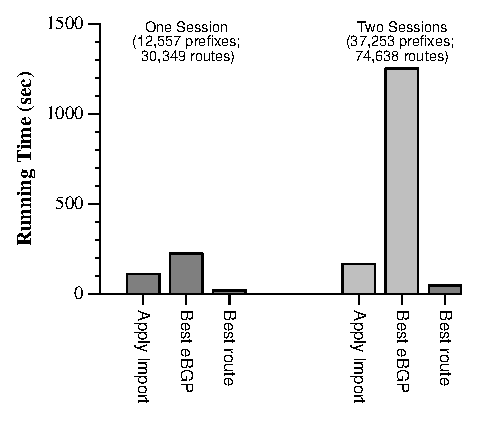
\epsfig{file=figures/peerperf.eps, height=1.75in, width=0.65\linewidth}
%% \caption{Performance of the emulator for a smaller number of eBGP sessions} 
%% \label{fig:peerperf}
%% \end{figure}


%\subsection{Computing the Set of Best eBGP Routes}

%% \begin{table}[t]
%% \begin{small}
%% \begin{center}
%% \begin{tabular}{r|r|r|r}
%% & {\em Predictions} & {\em Time (sec)} & {\em Prefixes/sec}\\ \hline
%% Without caching & 92419 & 17537 & 5.27 \\  \hline 
%% With caching & 8091 & 12033 & 8.23 \\
%% \end{tabular}
%% \end{center}
%% \end{small}
%% \caption{Running times for the second module, which
%%   computes the set of 
%%   best eBGP routes. Recognizing that prefixes can be grouped according
%%   to how they are advertised produces a significant speedup.  
%% }
%% \label{tab:perf2}
%% \end{table}

%
%However, recognizing that groups of prefixes are often advertised in
%exactly the same fashion allows the emulator to avoid recomputing the
%best routes for prefixes that are equivalent in terms of where they are
%advertised, the attributes they are advertised with, etc.  
%and subsequently performs route prediction by figuring out which group
%of equivalent prefixes a particular prefix belongs to.  Then, the module
%checks its cache to determine if it has already computed the set of best
%eBGP routes for some prefix in the group. In the case of a cache hit,
%the module simply reuses the previously computed answer; otherwise, it
%performs the prediction algorithm from Figure~\ref{fig:ep_pseudo}.


%% Figure~\ref{fig:peerperf} shows the running times for the second module
%% with one and two eBGP sessions and caching enabled.  The speedup for a
%% small number of sessions is not as dramatic as for other modules,
%% because, even for a small number of prefixes, there is not a linear
%% reduction in the number of prefixes and routes.  Nevertheless, the
%% running times are considerably smaller than for a network as large as
%% AT\&T's. 

%% \subsection{Computing the Best Route at Each Router}

%% \begin{table}[t]
%% \begin{small}
%% \begin{center}
%% \begin{tabular}{r|r|r|r|r}
%% & {\em Hits} & {\em Misses} & {\em Time (sec)} & {\em prefixes/sec}\\ \hline
%% Without caching & --- & --- & 390 & 211.6 \\ \hline 
%% With caching    & 82245 & 290 & 245 & 336.9 \\ 
%% \end{tabular}
%% \end{center}
%% \end{small} 
%% \caption{Running times and cache performance for the third module, which
%%   computes the best egress router. The results are 
%% from the validation of RR1, where predictions are made for 82,535
%% prefixes. This is one less than the 82,536 prefixes that we 
%% validated, as one prefix had an empty egress set (a Case 1 error for
%%   which we could not make a prediction).
%% }
%% \label{tab:perf3} 
%% \end{table}

%% Table~\ref{tab:perf3} shows the running time and cache performance for
%% the third module. The results come from the validation test of RR1
%% from Table~\ref{tab:predictions_summary}. The performance of the third
%% module is greatly improved by exploiting the nature of routing table
%% data.  For an ingress router, we only need to calculate the best
%% egress router for a given egress set once. Without caching, it takes
%% 390 seconds to predict the best egress router for the 82,535 prefixes
%% at this router, or about 212 prefixes per second. 

%Figure~\ref{fig:peerperf} shows that module 3's running time is
%comparatively small: 19 seconds and 47 seconds for one and two eBGP
%sessions, respectively. 
